\chapter{Conceituação Teórica}\label{cap2}



\section{Extração de Tópicos}

Os modelos de extração de tópicos foram propostos para simplificar e organizar grandes coleções de documentos. Nesse contexto, um tópico é uma estrutura com valor semântico que formam grupos de palavras que frequentemente ocorrem próximas. Essas palavra ajudam a descrever um documento ou sub-conjunto de documentos e ajudam a entender o tema ou assunto do texto onde essa estrutura está presente.

As técnicas de extração de tópicos são abordagens não-supervisionadas que visam encontrar a estrutura semântica de uma coleção de documentos a qual é latente, isto é, desconhecida. Os modelos de extração de tópicos baseiam-se na ideia de que um documento é produzido a partir de tópicos previamente definidos, os quais se deseja aborda no texto e determinam os termos a sem utilizados em um documento.

O processo de elaboração do documento a partir desses tópicos é chamado de processo generativo ou modelo generativo, o qual é desconhecido porém, pode ser estimado  com base nos termos presentes no documento, aqui chamados de variáveis observáveis. Assim, o processo de extração de tópicos consiste em estimar o modelo generativo que de origem ao documento.

Obtém-se ao final do processo de extração de tópicos uma representação documento-tópico que atribui um peso para cada tópico em cada documento da coleção e um representação termo-tópico que representa a probabilidade de ocorrência de um termo em um documento dado que o tópico está presente no documento.


Entre as principais abordagens da literatura está o Latent Dirichlet Allocation (LDA) sendo referenciado em diversos trabalhos e considerado um dos primeiros modelos dessa área e base para outros trabalhos. 




% Essas são técnicas não-supervisionadas, ou seja, os resultados são extraídos a partir da análise dos documentos sem a necessidade de informações extras como 


















		


% ==================== Segmentação ===================== %


\section{Segmentação Textual}


%%%%%%%%%%
% Definição da Tarefa
%%%%%%%%%%
A tarefa de segmentação textual consiste em dividir um texto em partes que contenham um significado relativamente independente. Em outras palavras, é identificar as posições nas quais há uma mudança significativa de assuntos. 

O interesse por segmentação textual tem crescido em em aplicações voltadas a recuperação de informação %citar o [15] ...
e sumarização de textos~\cite{Maziero2016}. %... e [2] do "Efficient Linear T S"
Essa técnica pode ser usada para melhorar o acesso a informação quando essa é solicitada por meio de uma consulta, onde é possível oferecer porções menores de texto mais relevantes ao invés de exibir um documento grande que pode conter informações menos pertinentes. 
%
Além disso, encontrar pontos onde o texto muda de assunto, pode ser útil como etapa de pré-processamento em aplicações voltadas ao entendimento do texto, principalmente em textos longos.
%
A navegação pelo documento pode ser aprimorada, em especial na utilização por usuários com deficiência visual, os quais utilizam  sintetizadores de texto como ferramenta de acessibilidade~\cite{Choi2000}. 
%
A sumarização de texto pode ser melhorada ao processar segmentos separados por tópicos ao invés de documentos inteiros~\cite{Bhatia2016, Maziero2016, Bokaei2016}. 




%  Descrição das Atas
%  
%  Ausência de marcaçãoes 
%  ... as lacunas
%  Diferenças de entre Línguas
As atas de reunião diferem dos textos comumente estudados em outros trabalhos em alguns pontos. O estilo de escrita mais sucinto, com poucos detalhes dificulta o processo de segmentação~\cite{Choi2001-LSA}. Há também um maior foco no idioma inglês, presente na maioria dos artigos publicados. Embora haja abordagens voltadas para outros idiomas, falta ainda uma maior atenção na literatura sobre língua portuguesa e a documentos com características próprias como as atas de reunião. Diferenças de performance podem ser vistas no mesmo algoritmo quando aplicado em documentos de diferentes idiomas, onde a aplicação em textos em inglês apresenta um taxa de erro significativamente menor que o alemão e o espanhol~\cite{Kern2009,Sitbon2004}.



 % =======================================================


Um segmento pode ser visto como uma sucessão de unidades de informação que compartilham o mesmo assunto e cada ponto entre duas unidades é considerado um candidato a limite entre segmentos.


%  Coesão léxica como **presuposto básico**
Trabalhos anteriores se apoiam na ideia de que a mudança de tópicos em um texto é acompanhada de uma proporcional mudança de vocabulário. Essa ideia, chamada de coesão léxica, sugere que a distribuição das palavras é um forte indicador da estrutura do texto. A partir disso, vários algoritmos foram propostos baseados na ideia de que um segmento pode ser identificado pela análise das palavras que o compõe~\cite{Chen2017,Ferret2009,Sakahara2014}.


%  Porque cosseno
Uma vez que a coesão léxica é pressuposto básico da maioria dos algoritmos, o cálculo da similaridade entre unidades de informação é fundamental. Uma medida de similidade frequentemente utilizada é o cosseno, apresentada na Equação~\ref{equ:cosine}, onde $f_{x,j}$ é a frequência da palavra $j$ na sentença $x$ e $f_{y,j}$ é a frequência da palavra $j$ na sentença $y$.
				

\begin{equation}
Sim(x,y) = \frac
{\Sigma_j f_{x,j} \times f_{y,j}}
{\sqrt{\Sigma_j f^2_{x,j} \times \Sigma f^2_{y,j}}}
\label{equ:cosine}
\end{equation}


\subsection{Principais algoritmos}
	\label{subsec:principaisalgoritimos}

Entre os principais trabalhos da literatura podemos citar o  \textit{TextTiling}~\cite{Hearst1994} e o \textit{C99}~\cite{Choi2000}.
%
%%%%%%%%%%%%%%%%%%%%%%%%%%%%%%%%%%%%%%%%%%%%%%%
%%%              TextTiling                 %%%
%%%%%%%%%%%%%%%%%%%%%%%%%%%%%%%%%%%%%%%%%%%%%%%
O \textit{TextTiling} é um algoritmo baseado em janelas deslizantes, em  que, para cada candidato a limite, analisa-se o texto circundante. Um limite ou quebra de segmento é identificado sempre que a similaridade cai abaixo de um limiar.
% \textit{threshold}. %TODO - explicar como se encontra os vales

O \textit{TextTiling} recebe uma lista de candidatos a limite, usualmente finais de parágrafo ou finais de sentenças. Para cada posição candidata são construídos 2 blocos, um contendo sentenças que a precedem e outro com as que a sucedem. O tamanho desses blocos é um parâmetro a ser fornecido ao algoritmo e determina o tamanho mínimo de um segmento.
%
Em seguida, os blocos de texto são representados por vetores que contém as frequências de suas palavras. Então, usa-se cosseno (Equação~\ref{equ:cosine}) para calcular a similaridade entre os blocos adjacentes a cada candidato e identifica-se uma transição entre tópicos pelos vales na curva de dissimilaridade.
%TODO como apresentado na Figura~\ref{fig:curvadedissimilaridade}.

O \textit{TextTiling} possui baixa complexidade computacional. Por outro lado, algoritmos mais complexos, como os baseados em matrizes de similaridade, apresentam acurácia relativamente superior como apresentado em~\cite{Choi2000, Kern2009, Misra2009}.




%%%%%%%%%%%%%%%%%%%%%%%%%%%%%%%%%%%%%%%%%%%%%%%
%%%                  C99                    %%%
%%%%%%%%%%%%%%%%%%%%%%%%%%%%%%%%%%%%%%%%%%%%%%%

O C99 é um algoritmo baseado em ranking.
% Choi \cite{Choi2000} apresenta um algoritmo baseado em ranking, o \textit{C99}. 
%
Embora muitos trabalhos utilizem matrizes de similaridades para pequenos segmentos, o cálculo de suas similaridades não é confiável, pois uma ocorrência adicional de uma palavra causa um impacto que pode alterar significativamente o cálculo da similaridade~\cite{Choi2000}.
%
Além disso, o estilo da escrita pode não ser constante em todo o texto. Por exemplo, textos iniciais dedicados a introdução costumam apresentar menor coesão do que trechos dedicados a um tópico específico. Portanto, comparar a similaridade entre trechos de diferentes regiões não é apropriado.
% Complexidade O(n²)
Devido a isso, as similaridades não podem ser comparadas em valores absolutos. Então, contorna-se esse problema fazendo uso de \textit{rankings} de similaridade para encontrar os segmentos de texto. 


Inicialmente é construída uma matriz que contém as similaridades de todas as unidades de texto. Em seguida, cada valor na matriz de similaridade é substituído por seu ranking local. Para cada elemento da matriz, seu \textit{ranking} é o número de elementos vizinhos com valor de similaridade menor que o seu.
% O que é a máscara
Então, cada elemento e comparado com seus vizinhos dentro de uma região denominada máscara.
%

Na Figura~\ref{fig:a} é destacado um quadro 3~x~3 de uma matriz em que cada elemento é a similaridade entre duas unidades de informação. 
%
Tomando como exemplo o elemento com valor $0,5$, a mesma posição na matriz de \textit{rankings} terá o valor $4$, pois esse é o número de vizinhos com valores inferiores a $0,5$ dentro do quadro analisado na matriz de similaridades. Da mesma forma, na Figura~\ref{fig:b} para o valor $0,2$ a matriz de \textit{rankings} conterá o valor $1$ na mesma posição.


% Na Figura~\ref{fig:exemplomatrixrank} é apresentado um quadro de dimensões 3~x~3 destacado na matriz de similaridades, que contém os valores $\{0,3; 0,4; 0,4; 0,6; 0,5; 0,2; 0,9; 0,5; 0,7\}$, onde cada elemento da matriz é a similaridade entre duas unidades de informação. Tomando como exemplo o elemento com valor $0,5$, a mesma posição na matriz de \textit{ranks} terá o valor $4$, pois esse é o número de vizinhos com valores inferiores a $0,5$ dentro do quadro analisado na matriz de similaridades. 



\begin{figure}[!h]
	\centering     %%% not \center

	\subfigure[Passo 1]{\label{fig:a}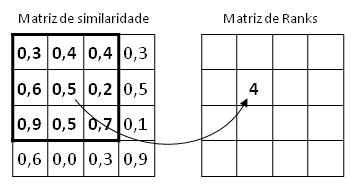
\includegraphics[width=60mm]{conteudo/capitulos/figs/exemplo-matrix-rank-A.png}}
	\subfigure[Passo 2]{\label{fig:b}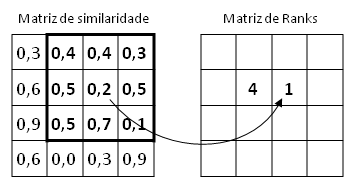
\includegraphics[width=60mm]{conteudo/capitulos/figs/exemplo-matrix-rank-B.png}}
	
	\caption{Exemplo de construção de uma matriz de rankings.%~\cite{Choi2000}.
	}
	\label{fig:exemplomatrixrank}
\end{figure}



Finalmente, com base na matriz de \textit{rank}, o \textit{C99} utiliza um método de \textit{clustering} baseado no algoritmo de maximização de Reynar
% ~\cite{Reynar1998} 
para identificar os limites entre os segmentos. 





\subsection{Avaliação}





\subsubsection{Medidas de Avaliação}

%  Medidas de avaliação tradicionais 
As medidas de avaliação tradicionais como precisão e revocação 
computam os erros do algoritmo, isto é, falsos positivos e falsos negativos, a fim de calcular seu desempenho. 
Além dessas medidas, que consideram apenas se um segmento foi corretamente definido, pode-se também considerar a distância entre o segmento extraído automaticamente e o segmento de referência~\cite{Kern2009}. Chama-se \textit{near misses} o caso em que um limite identificado automaticamente não coincide exatamente com a referência, mas é necessário considerar a proximidade entre eles.



%  Medidas que consideram a distancia entre os segmentos 
Na Figura~\ref{fig:exemplosegmentacaozoom} é apresentado um exemplo com duas segmentações extraídas automaticamente e uma referência. Em ambos os casos não há nenhum verdadeiro positivo, o que implica em zero para os valores de precisão, acurácia, e revocação, embora a segunda hipótese possa ser considerada superior à primeira se levado em conta a proximidade dos limites.


  \begin{figure}[!h]

	\centering
	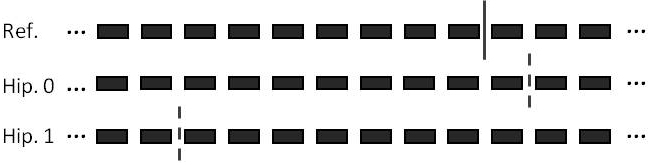
\includegraphics[width=0.6\textwidth]{conteudo/capitulos/figs/windiffzoom.jpg}
	\caption{Exemplos de \textit{near missing} e falso positivo puro. Os blocos indicam uma unidade de informação e as linha verticais representam uma transição de assunto. }
	\label{fig:exemplosegmentacaozoom}

  \end{figure}
  

Considerando o conceito de \textit{near misses}, algumas soluções foram propostas. As medidas de avaliação mais utilizadas são a P$_k$ e \textit{WindowDiff}.
% 
% 
% 
% 
%%%%%%%%%%%%%%%
% Pk 
%%%%%%%%%%%%%%% 
%\item Em~\cite{Beeferman1999} é apresentada uma medida denominada P$_k$, 
% Valores Parciais 
% Funcionamento 
% Compara hipotese e referência		
% Penalisa em caso de discrepânica 
% Calculo de k 
% Medida de dissimilaridade e interpretação 

 
Proposta por~\cite{Beeferman1999}, P$_k$, atribui valores parciais a \textit{near misses}, ou seja, limites sempre receberão um peso proporcional à sua proximidade, desde que dentro de um janela de tamanho~$k$.  Para isso, esse método move uma janela de tamanho $k$ ao longo do texto.  A cada passo verifica, na referência e na hipótese, se o início e o final da janela estão ou não dentro do mesmo segmento, então, penaliza o algoritmo caso não concorde com a referência. Ou seja, dado duas palavras de distância $k$, o algoritmo é penalizado quando não concordar com a segmentação de referência se as palavras estão ou não no mesmo segmento.  O valor de $k$ é calculado como a metade da média dos comprimentos dos segmentos reais. Como resultado, é retornado a contagem de discrepâncias divida pelo quantidade de segmentações analisadas.  P$_k$ é uma medida de dissimilaridade entre as segmentações e pode ser interpretada como a probabilidade de duas sentenças extraídas aleatoriamente pertencerem ao mesmo segmento.




%%%%%%%%%%%%%%%
% WindowDiff 
%%%%%%%%%%%%%%% 
%Em \cite{Pevzner2002} 
% Medida alternativa que considera outros aspectos 
% Funcionamento do Windiff 
% Solução para considerar o tamanho das sentenças 
% Solução para equilibrar falsos positivos e near missses 
\textit{WindowDiff} é uma medida alternativa à P$_k$. % a fim de melhorar alguns aspectos. 
De maneira semelhante, move uma janela pelo texto e penaliza o algoritmo sempre que o número de limites proposto pelo algoritmo não coincidir com o número de limites esperados para aquela janela. Ou seja, o algoritmo é penalizado quando não concordar com a segmentação de referência quanto ao número de segmentos na janela.  Assim, consegue manter a sensibilidade a \textit{near misses} e além disso, considerar o tamanho das janelas.  A fim de melhor equilibrar o peso dos falsos positivos em relação a \textit{near misses}, dobra-se a penalidade para falsos positivos, evitando-se a supervalorização dessa medida. 
% OBS: Os problemas de Pk ficaram subentendidos aqui :/ 







As medidas de avaliação tradicionais, como acurácia, precisão e revocação, podem não ser confiáveis, por não considerarem a distância entre os limites, mas penalizam o algoritmo sempre que um limite que não coincide perfeitamente com a referência. Essas medidas podem ser mais adequadas quando necessita-se de segmentações com maior exatidão. 


As medidas \textit{WindowDiff} e P$_k$, consideram a quantidade e proximidade entre os limites, sendo mais tolerantes a pequenas imprecisões. Essa é uma característica desejável, visto que as segmentações de referência possuem diferenças consideráveis. 
%
\textit{WindowDiff} equilibra melhor os falsos positivos em relação a \textit{near misses}, ao passo que P$_k$ os penaliza com peso maior. Isso significa que segmentadores melhores avaliados em P$_k$ ajudam a selecionar as configurações que erram menos ao separar trechos de texto com o mesmo assunto, enquanto \textit{WindowDiff} é mais tolerante nesse aspecto.

Observa-se  melhores resultados de \textit{WindowDiff} quando os algoritmos aproximam a quantidade de segmentos automáticos da quantidade de segmentos da referência. %em torno de 10. 
Por outro lado, observa-se que P$_K$ avalia melhor as configurações que retornam menos segmentos. A configuração do tamanho do passo (P) e da proporção de segmentos em relação ao número de candidatos (S), influenciam os algoritmos na quantidade de segmentos extraídos. Contudo, não é possível definir um valor adequado, uma vez que os segmentadores humanos frequentemente apontam valores diferentes.




% De maneira geral, o algoritmo \textit{C99} apresentou melhores resultados em relação ao \textit{TextTiling}, contudo, testes estatísticos realizados indicaram que não houve diferença significativa entre os métodos. A etapa de pré-processamento proporciona melhora de desempenho quando aplicada, porém o seu maior benefício é a diminuição do custo computacional, uma vez que não prejudica a qualidade dos resultados.


































